% Standalone pgfplots figure -- compile directly with pdflatex/lualatex,
% or \input{<this file>} into a document that loads \usepackage{pgfplots}.
% bb144 d=12 circuit-level LER vs p (p-bit ColoredBlockGibbsDecoder).
% NOTE: p=0.001 preliminary (campaign ongoing 2026-06-25)
\documentclass[tikz,border=3mm]{standalone}
\usepackage{pgfplots}
\pgfplotsset{compat=1.17}
\begin{document}
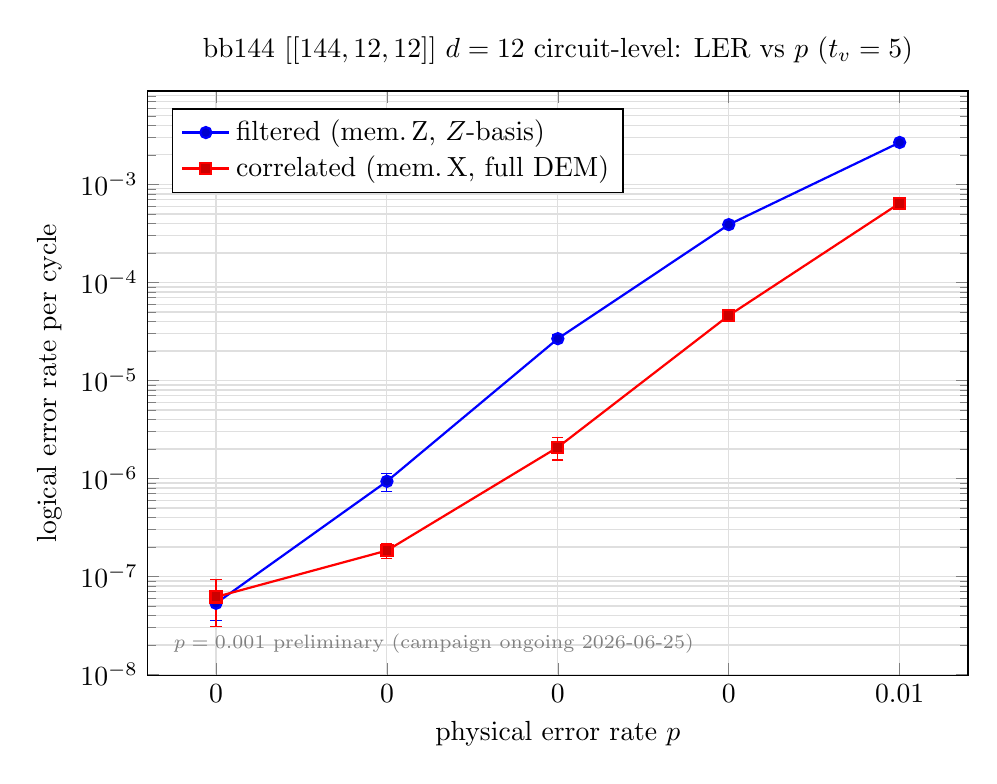
\begin{tikzpicture}
\begin{semilogyaxis}[
    width=12cm, height=9cm,
    xlabel={physical error rate $p$},
    ylabel={logical error rate per cycle},
    title={bb144 $[[144,12,12]]$ $d=12$ circuit-level: LER vs $p$ ($t_v=5$)},
    xtick={0.001,0.002,0.003,0.004,0.005},
    scaled x ticks=false, x tick label style={/pgf/number format/fixed},
    grid=both, grid style={gray!25},
    legend pos=north west, legend cell align=left,
    mark options={solid}, every axis plot/.append style={thick},
]
\addplot+[color=blue, mark=*, error bars/.cd, y dir=both, y explicit]
    coordinates {(0.001, 5.3267e-08) +- (0, 1.7758e-08) (0.002, 9.3583e-07) +- (0, 1.9167e-07) (0.003, 2.6692e-05) +- (0, 2.4167e-06) (0.004, 3.8933e-04) +- (0, 2.2500e-05) (0.005, 2.6825e-03) +- (0, 1.8333e-04)};
\addlegendentry{filtered (mem.\,Z, $Z$-basis)}
\addplot+[color=red, mark=square*, error bars/.cd, y dir=both, y explicit]
    coordinates {(0.001, 6.1908e-08) +- (0, 3.0950e-08) (0.002, 1.8407e-07) +- (0, 3.2042e-08) (0.003, 2.0833e-06) +- (0, 5.3792e-07) (0.004, 4.6007e-05) +- (0, 6.3195e-06) (0.005, 6.4352e-04) +- (0, 5.4583e-05)};
\addlegendentry{correlated (mem.\,X, full DEM)}
\node[anchor=south west, font=\scriptsize, text=gray]
    at (rel axis cs:0.02,0.02) {$p=0.001$ preliminary (campaign ongoing 2026-06-25)};
\end{semilogyaxis}
\end{tikzpicture}
\end{document}
